\documentclass{article}
\usepackage[utf8]{inputenc}
\usepackage{graphicx}
\title{Bohr's Theory of Hydrogen Atom and Hydrogen Spectra}
\author{Arsham Eghdamian } % Author name

\date{\today} % Date for the report

\begin{document}

\maketitle % Insert the title, author and date

\begin{center}
\begin{tabular}{l r}
Date Performed: & January 27, 2016 \\ % Date the experiment was performed
Partners: & Whole class \\ % Partner names
Instructor: & Dr. Schultz % Instructor/supervisor
\end{tabular}
\end{center}


\maketitle

Bohr’s theory of Hydrogen suggests that there are discrete energy levels around atom that electrons can take on electrons are naturally at the ground level but when its given a certain energy levels which corresponds to the difference of energy levels around the Hydrogen atom the electron can magically (without traveling in between the levels) appear at the upper level and it eventually releases its energy in order to get to the ground state and become stable. Electrons release the energy through photons and each photon has a different energy, therefore a different wavelength and color. The picture below demonstrates the emitted photons received by a Hydrogen gas when its electron is being exited. This is called spectrum and the method of collecting these lines is spectroscopy. 
\begin{figure}[h!]
    \centering
    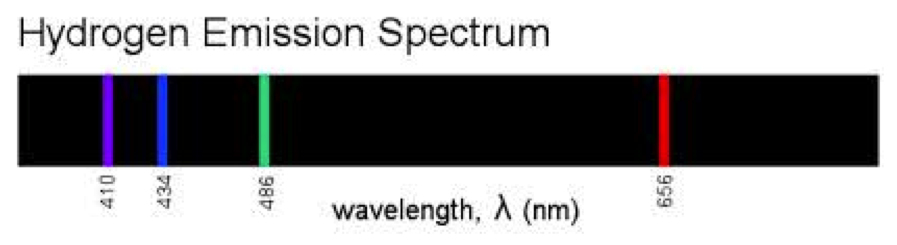
\includegraphics[scale=0.7]{HE.png}
    
\end{figure}
Although electrons are particles but they act like waves based on quantum theory. This is shown by DeBroglie relationship. In fact based on DeBroglie relationship and quantum theory we all have wavelengths but because of are big mass and the very small value of planks constant it doesn’t affect our daily lives. 
\begin{equation}
    \lambda = \frac{h}{mv}
\end{equation}
	
Although electrons are particles but they act like waves based on quantum theory. This is shown by DeBroglie relationship. In fact based on DeBroglie relationship and quantum theory we all have wavelengths but because of are big mass and the very small value of planks constant it doesn’t affect our daily lives. \\

On the other hand scientists realized that electrons movement around atoms is like standing waves and we know that. $L=n\lambda$\\
\begin{equation}
    L=2\pie{r}=n\lambda \rightarrow E_{K}=\frac{1}{2}mv^{2}
\end{equation}
\begin{figure}[h!]
    \centering
    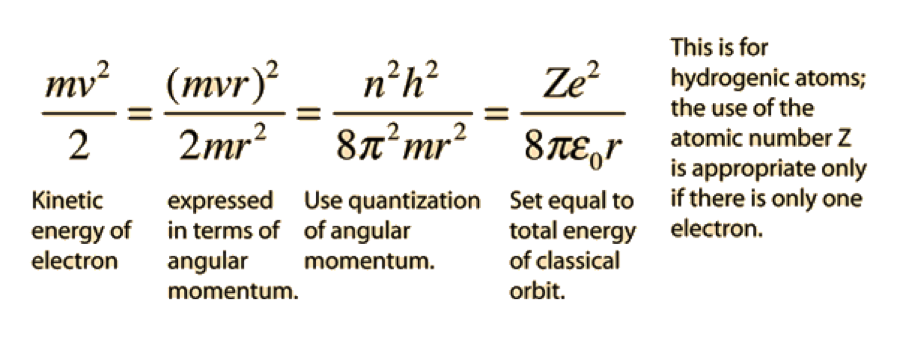
\includegraphics{E1.png}
\end{figure}
\begin{figure}[h!]
    \centering
    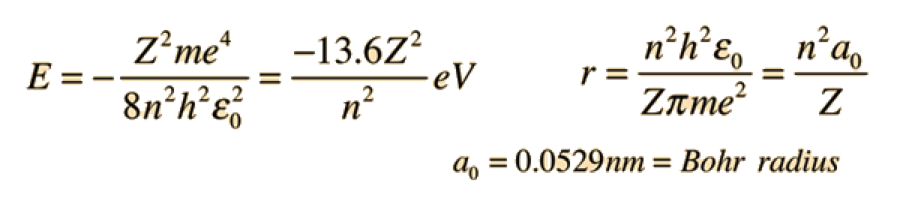
\includegraphics{E2.png}
\end{figure}\\
Now we know that the energy for each level is $E=\frac{-13.6z^{2}}{n^{2}}eV$ We can calculate the energy of those emitted lights by subtracting one level from the other :\\
\begin{equation}
    E=-13.6z^{2}(\frac{1}{n^{2}}-\frac{1}{m^{2}}) eV
\end{equation}
Now that we have the Energy difference of layers we can find the wavelength of those emitted lines by using the formula of 
\begin{equation}
    E=hf=\frac{hc}{\lambda}
\end{equation}
\begin{figure}[h!]
    \centering
    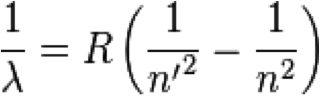
\includegraphics{E3.png}
\end{figure}\\

The lines that were observed in the emission spectra of hydrogen were the result of transition of electrons from 3-2 (Alpha –Hydrogen) , 4-2(Beta) , 5-2(Gamma) 
\end{document}
